\documentclass[conference]{IEEEtran}

\usepackage{amsmath,amssymb}
\usepackage{graphicx}
\usepackage{booktabs}
\usepackage{tabularx}
\usepackage{xcolor}
\usepackage[hidelinks]{hyperref}
\usepackage{cite}
\usepackage{pgfplots}
\pgfplotsset{compat=1.18}

% Palette matched to the project wordmark (assets/logo-*.svg): accent green for
% libaio, the baseline that wins outright, then three more hues distinct enough
% to separate on a grayscale printout via marker and line-style alone.
\definecolor{cLibaio}{HTML}{22C55E}
\definecolor{cPlainUring}{HTML}{3B82F6}
\definecolor{cSqpollIndep}{HTML}{F59E0B}
\definecolor{cSqpollShared}{HTML}{8B5CF6}
\definecolor{cBox4}{HTML}{94A3B8}
\definecolor{cBox16}{HTML}{1E293B}

\begin{document}

\title{Measuring the Limits of SQPOLL \texttt{io\_uring}\\for NVMe I/O}

\author{
  \IEEEauthorblockN{Parth}
  \IEEEauthorblockA{\texttt{sinhaparth555@gmail.com}}
}

\maketitle

\begin{abstract}
Kernel-bypass storage designs built on Linux \texttt{io\_uring}'s \texttt{IORING\_SETUP\_SQPOLL}
mode are motivated by a simple argument: a dedicated kernel polling thread removes the
per-operation syscall that blocking and non-polling asynchronous I/O interfaces pay, so on
modern NVMe hardware, where flash latency is no longer the bottleneck, SQPOLL should win on
throughput. We built \texttt{ringio}, a header-only C++20 storage engine around this argument,
and tested it against \texttt{libaio} and plain \texttt{io\_uring} (no SQPOLL) on real NVMe
across two machine sizes (4 and 16 vCPUs) and a swept queue-depth and thread-count matrix. The
argument does not hold in our measurements. At matched thread count and queue depth, SQPOLL does
not beat the syscall-based baselines on raw IOPS at either machine size, ruling out core
oversubscription as the explanation. \texttt{libaio}'s advantage over SQPOLL widens, not narrows,
on the wider box, and SQPOLL's tail latency degrades under more available cores rather than
improving. What SQPOLL does deliver is a large reduction in kernel entries per completed
operation, roughly an order of magnitude fewer than plain \texttt{io\_uring} at high queue depth,
at the cost of that added tail latency. We report the full methodology, including a
page-cache measurement defect that invalidated an earlier round of results, and discuss what
this suite's data does and does not establish about the underlying cause.
\end{abstract}

\begin{IEEEkeywords}
io\_uring, SQPOLL, kernel-bypass I/O, NVMe, storage engine, asynchronous I/O, benchmarking
\end{IEEEkeywords}

\section{Introduction}

Asynchronous storage interfaces on Linux have moved through several generations: blocking
\texttt{read}/\texttt{write}, POSIX AIO, \texttt{libaio}, and now \texttt{io\_uring}. Each
generation targets the same cost: a syscall is a mode switch, and a mode switch is expensive
relative to the latency of an NVMe device, whose flash media now services a random 4KB
operation in tens of microseconds. \texttt{io\_uring}'s \texttt{IORING\_SETUP\_SQPOLL} mode goes
further than reducing the number of syscalls per operation; run with a dedicated kernel polling
thread, submitting a request can become a plain memory write with no syscall at all, as long as
that polling thread has not gone idle.

This is the design bet behind \texttt{ringio}, a header-only C++20 asynchronous storage engine
we built around SQPOLL: a lock-free multi-producer multi-consumer ring feeds fixed, pre-registered
buffers into an SQPOLL \texttt{io\_uring} instance, with completions harvested and correlated back
to requests by an opaque token. The design followed directly from the argument above. We report
here what testing it against real hardware actually found, which is not what the argument
predicts.

Three findings structure this paper. First, an SQPOLL kernel poller is not free: it busy-spins
continuously and costs a full CPU core by itself, so an SQPOLL ring is a two-core commitment, not
one, and a naive one-ring-per-thread design collapses once thread count approaches the machine's
core count. Sharing one poller across many rings fixes this specific collapse. Second, once that
fix is in place and the benchmark harness is corrected to bypass the page cache and pipeline
requests to a real queue depth, SQPOLL still does not win on raw IOPS against \texttt{libaio} or
plain \texttt{io\_uring} at any matched thread count and queue depth we tested, on either a
4-vCPU or a 16-vCPU machine. Third, the widening of \texttt{libaio}'s lead and the growth in
SQPOLL's tail latency when we moved from 4 to 16 vCPUs rules out core oversubscription as the
explanation for the second finding, leaving the actual cause unresolved by this suite's data.

We present the full experimental record, including a page-cache measurement defect in an early
version of the harness that produced DRAM-speed numbers mislabeled as disk I/O, because the
defect and its fix are as much a part of what this work establishes as the final results are.

\section{Background}

\subsection{io\_uring and SQPOLL}

\texttt{io\_uring} exposes two ring buffers shared between user space and the kernel: a
submission queue (SQ) and a completion queue (CQ). In its default mode, a thread still issues
\texttt{io\_uring\_enter} to tell the kernel new submission queue entries (SQEs) are ready, and
to wait for completion queue entries (CQEs); this call is a syscall, though one call can carry
many requests, unlike \texttt{read}/\texttt{write} pairs.

\texttt{IORING\_SETUP\_SQPOLL} changes this: the kernel spawns a dedicated thread that polls the
SQ continuously. As long as that thread has not gone idle for longer than a configurable
\texttt{sq\_thread\_idle} window, writing a new SQE and advancing the SQ tail is enough for the
kernel poller to pick it up. No \texttt{io\_uring\_enter} call is required on the submission
side. Waiting for completions can still avoid a syscall if the caller polls the CQ head
non-blockingly instead of waiting on it.

\subsection{libaio and plain io\_uring without SQPOLL}

\texttt{libaio} is the older Linux asynchronous I/O interface, backed by
\texttt{io\_submit}/\texttt{io\_getevents}. Both are syscalls, but each call can carry a batch of
operations, so the per-operation cost is amortized across the batch size rather than eliminated.
Plain \texttt{io\_uring}, used here without SQPOLL, has the same syscall-per-round-trip structure
as \texttt{libaio} but through \texttt{io\_uring\_enter} instead: it batches submission and
completion but still crosses into the kernel to do either.

\subsection{O\_DIRECT and the page cache}

Every I/O interface discussed here can be measured incorrectly if the target file is not opened
with \texttt{O\_DIRECT}. Without it, the kernel serves reads from the page cache once a block has
been read once, and buffers writes in the page cache before flushing them to the device later.
A benchmark against a small working set on a machine with enough RAM to hold it will then measure
DRAM bandwidth and latency, not the storage device's. \texttt{O\_DIRECT} requires the buffer
address, transfer length, and file offset to all be aligned to the device's logical block size
(4096 bytes on the hardware used here); an unaligned request fails with \texttt{EINVAL}.

\section{System Design}

\texttt{ringio} is built from three components, added in dependency order. A lock-free
multi-producer multi-consumer ring (\texttt{MpmcRing}, and a single-producer variant,
\texttt{SpscRing}) carries trivially copyable request structs from worker threads into the
submission path. A buffer pool (\texttt{BufferPool}) allocates a fixed set of page-aligned
buffers via \texttt{posix\_memalign}, locks them with \texttt{mlock}, and registers them with
the kernel once via \texttt{io\_uring\_register\_buffers}, so I/O against them avoids
per-request page pinning. \texttt{SqpollEngine} owns one SQPOLL \texttt{io\_uring} instance,
registers fixed file descriptors once via \texttt{io\_uring\_register\_files}, drains a batch of
requests from either ring type into real SQEs, and harvests finished CQEs non-blockingly into a
completion ring, matching each one back to its request by a 64-bit token.

\subsection{The two-core cost of a poller}

An SQPOLL kernel thread busy-spins for as long as it stays awake, which means it occupies a full
CPU core regardless of how much work is actually arriving. One \texttt{SqpollEngine} is
therefore a two-core commitment: one core for the poller, one for whatever application thread
feeds it. A design that gives every worker thread its own engine, which is what "one ring per
thread" naturally suggests, runs out of core budget at half the machine's thread count. We found
this directly: on a 4-vCPU machine, independent rings collapsed from 157K IOPS at 2 threads to
71K at 8 threads.

\texttt{SqpollEngine}'s constructor takes an optional \texttt{attach\_to} parameter. When set,
the new engine shares \texttt{attach\_to}'s kernel poller via \texttt{IORING\_SETUP\_ATTACH\_WQ}
instead of spawning its own; each attached engine still owns its own SQ/CQ ring pair, but the
kernel services all of them from one polling thread. $N$ engines sharing one poller then cost
$1 + N$ cores instead of $2N$. On the same 4-vCPU machine, threads sharing one poller climbed to
248K IOPS at 8 threads and had not plateaued, instead of collapsing.

\subsection{Completion-side backoff}

The first version of the shared-poller benchmark undersold this fix: its worker threads
harvested completions in a flat busy-spin loop, so every application thread burned a full core on
top of the one core the shared poller itself occupies, reintroducing a collapse from the
application side even though the kernel mechanism no longer had one. Replacing the flat spin with
a three-tier backoff (fast retries, then bounded pause-instruction spinning, then a scheduler
yield) let a waiting thread give cycles back to the scheduler instead of denying it, which the
poller needs to actually run. This did not create CPU capacity that was not there; the
shared-poller numbers still peaked at 2 threads on the 4-vCPU box and declined afterward, since 4
vCPUs means 1 core for the poller and 3 for application threads. What backoff fixed was the
collapse being disproportionate to that oversubscription: at 8 threads, throughput before the fix
fell to 46K IOPS; after it, the same configuration held 112K.

\section{Methodology}

We benchmark five backends against the same workload: 4KB random reads and writes, alternating,
against a 1\,GiB working set, on a scratch file opened with \texttt{O\_DIRECT}. The five
backends are POSIX \texttt{pread}/\texttt{pwrite}, \texttt{libaio}, plain \texttt{io\_uring}
without SQPOLL, \texttt{SqpollEngine} with one independent poller per thread, and
\texttt{SqpollEngine} with every thread past the first attached to a single shared poller. Each
backend uses its own file descriptor, buffers, and (where applicable) ring per thread; concurrent
\texttt{io\_uring\_submit} calls against one shared SQ ring from multiple threads are not safe
without locking \texttt{ringio} does not provide, so per-thread instances are the correct
comparison rather than a shortcut. \texttt{SqpollEngine}'s buffers are pre-registered,
page-locked, and addressed as fixed buffers, matching how the design is meant to run; the three
baselines use heap memory aligned only as far as \texttt{O\_DIRECT} requires. Each backend is
measured at its own best practice, not with identical buffer handling forced across all five.

\subsection{Queue-depth pipelining}

\texttt{libaio}, plain \texttt{io\_uring}, and both \texttt{SqpollEngine} variants keep a
configurable number of requests, the queue depth, in flight at once: submit a batch, reap
completions as they land, and resubmit immediately, rather than the submit-one-block-wait-one
loop an earlier version of this harness used. We sweep queue depth over
$\{1, 8, 32, 64, 128\}$. POSIX \texttt{pread}/\texttt{pwrite} has no queue-depth axis: it is a
blocking syscall with nothing to submit ahead of, and its thread-count sweep already covers the
concurrency dimension a synthetic queue-depth parameter on a blocking call would otherwise
duplicate.

\subsection{Thread-count sweep and its bound}

POSIX runs the full $\{1, 2, 4, 8, 16, 32\}$ thread sweep, since it costs nothing extra and has
no queue-depth axis to cross it against. The four pipelined backends are swept at
$\{1, 2, 4, 8\}$ threads against the full queue-depth set; crossing the full 1--32 thread range
against the full queue-depth range for four backends would be 30 combinations each, more
provisioned-VM time than the question needs. $\{1, 2, 4, 8\}$ was chosen specifically to test
whether a result changes as thread count moves from well under to well past a small machine's
core budget, which is the question Section~V-D exists to answer.

\subsection{calls\_per\_op is an upper bound for the io\_uring-based backends}

We report a \texttt{calls\_per\_op} counter alongside IOPS and latency: submit calls plus reap
calls, divided by completed operations. For POSIX and \texttt{libaio} this is an exact syscall
count, since \texttt{pread}, \texttt{pwrite}, \texttt{io\_submit}, and \texttt{io\_getevents} are
unconditionally syscalls. For the \texttt{io\_uring}-based backends it is not:
\texttt{io\_uring\_submit} only issues a real \texttt{io\_uring\_enter} syscall when the SQPOLL
poller has gone idle, a check against a flag in the shared ring that is not visible from user
space. We report this figure as an upper bound on kernel entries for the three
\texttt{io\_uring}-based backends, not a confirmed syscall count.

\subsection{Hardware}

We provisioned short-lived GCE spot VMs for every run, one Local SSD NVMe device
(\texttt{interface=NVME}) bind-mounted over the benchmark's scratch directory, formatted
\texttt{ext4}, so \texttt{O\_DIRECT} reaches real flash rather than network-attached persistent
disk or, worse, a filesystem (tmpfs) that rejects \texttt{O\_DIRECT} outright. Two machine sizes
were used: an \texttt{n2-standard-4} (4 vCPUs) for the initial redesign and its results, and an
\texttt{n2-standard-16} (16 vCPUs, two Local SSD devices) for the wider-core rerun in
Section~V-D. Both ran at a fixed 2.8\,GHz per vCPU with frequency scaling disabled. Every VM was
deleted immediately after its run.

\section{Results}

\subsection{The page-cache measurement defect}

An earlier version of this harness opened its scratch file without \texttt{O\_DIRECT} against a
64\,MiB working set. On a VM with far more RAM than that, every backend's I/O after the first
pass was served from the page cache, not the NVMe device. POSIX \texttt{pread}/\texttt{pwrite}
reached 698K--1.3M IOPS in that run, which is DRAM bandwidth, not disk I/O; none of the baselines
in that round of results had touched the drive the suite claimed to measure. We report this
because a benchmark suite that silently measures the wrong subsystem is a common and
under-reported failure mode in storage system evaluation, not because the number itself is
otherwise interesting.

\subsection{4 vCPUs, O\_DIRECT, and queue-depth pipelining}

With \texttt{O\_DIRECT} and pipelining both in place, every backend's ceiling dropped to roughly
200K IOPS, a plausible figure for a virtualized NVMe device rather than DRAM speed. At matched
thread count and queue depth, plain \texttt{io\_uring} and \texttt{libaio} matched or beat both
\texttt{SqpollEngine} variants on raw IOPS. At 4 threads, plain \texttt{io\_uring} and
\texttt{libaio} both plateaued around 199--200K IOPS from queue depth 8 upward;
\texttt{SqpollEngine}'s best result at 4 threads was 135K (shared poller, queue depth 128). The
independent-ring variant did worse still, and reproduced the exact core-budget collapse from
Section~III-A at queue depth 1: 11.6K IOPS at 4 threads, down from 23.4K at 1 thread, the same
effect now visible across the queue-depth axis as well as the thread-count axis.

\begin{table}[t]
\centering
\caption{4 vCPUs, 4 threads, queue depth 128: round trips per operation
(\texttt{calls\_per\_op}) and p99 latency.}
\label{tab:4vcpu-calls}
\begin{tabular}{lrr}
\toprule
Backend & \texttt{calls\_per\_op} & p99 (ms) \\
\midrule
\texttt{libaio} & 1.3--4.3 & 14.3 \\
Plain \texttt{io\_uring} & 1.3--4.3 & 15.0 \\
\texttt{SqpollEngine} (independent) & 0.1--0.3 & 23.5 \\
\bottomrule
\end{tabular}
\end{table}

\begin{figure}[t]
\centering
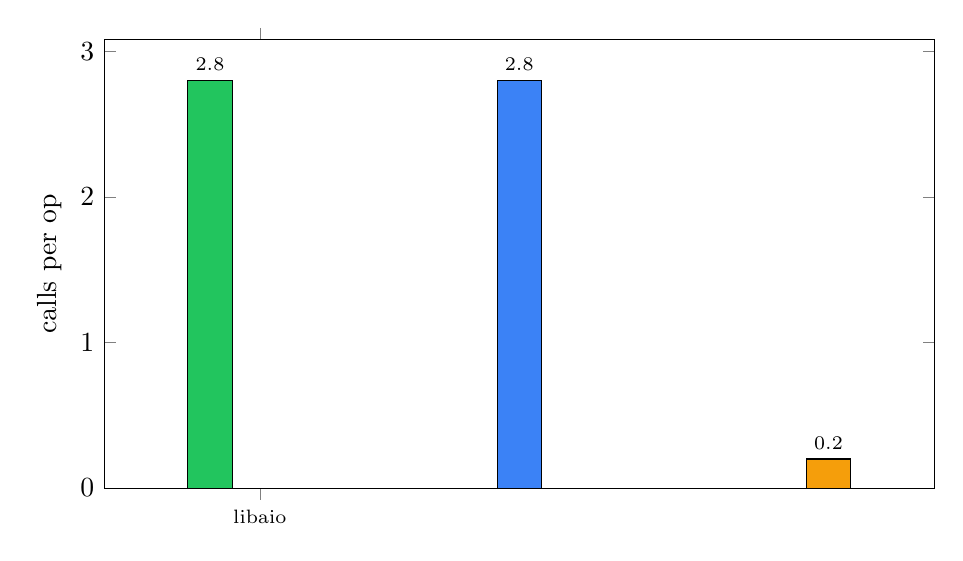
\begin{tikzpicture}
\begin{axis}[
    ybar,
    width=\linewidth,
    height=0.6\linewidth,
    symbolic x coords={libaio,plain io\_uring,SqpollEngine},
    xtick=data,
    x tick label style={font=\scriptsize},
    ylabel={calls per op},
    ymin=0,
    bar width=16pt,
    nodes near coords,
    every node near coord/.append style={font=\scriptsize},
    enlarge x limits=0.3,
]
\addplot[fill=cLibaio] coordinates {(libaio,2.8)};
\addplot[fill=cPlainUring] coordinates {(plain io\_uring,2.8)};
\addplot[fill=cSqpollIndep] coordinates {(SqpollEngine,0.2)};
\end{axis}
\end{tikzpicture}
\caption{Round trips per completed operation at 4 threads, queue depth 128. Bars for
\texttt{libaio} and plain \texttt{io\_uring} plot the midpoint of their reported 1.3--4.3 range;
Table~\ref{tab:4vcpu-calls} has the exact figures.}
\label{fig:calls-per-op}
\end{figure}

Table~\ref{tab:4vcpu-calls} shows where SQPOLL's design does pay off: at queue depth 128,
\texttt{SqpollIops} needs roughly an order of magnitude fewer round trips per completed
operation than plain \texttt{io\_uring} at the same setting. This is the batching mechanism
working as designed. It comes at a tail-latency cost: at 4 threads and queue depth 128,
\texttt{SqpollIops}'s p99 latency is 23.5\,ms, worse than plain \texttt{io\_uring}'s 15.0\,ms or
\texttt{libaio}'s 14.3\,ms at the identical setting. SQPOLL is spending fewer syscalls but
queuing completions longer before a harvesting thread picks them up.

The finding this round of data supports is narrower than "SQPOLL wins": fewer round trips per
operation, not more throughput, and worse tail latency at depth, on this hardware. Whether that
is inherent to the design or an artifact of this box's poller-versus-worker core split, 4 worker
threads and 1 poller thread contending for 4 physical cores, was open at this point in the
investigation.

\subsection{16 vCPUs: ruling out core oversubscription}

To separate those two explanations, we widened the thread-count sweep to $\{1, 2, 4, 8\}$ and
reran the full matrix on an \texttt{n2-standard-16}, giving every configuration up to 8 worker
threads plus the SQPOLL poller thread room across 16 vCPUs, instead of contending for 4.

\begin{table}[t]
\centering
\caption{16 vCPUs, queue depth 32: IOPS (thousands) by backend and thread count.}
\label{tab:16vcpu-qd32}
\begin{tabular}{lrrrr}
\toprule
Backend & 1 thr & 2 thr & 4 thr & 8 thr \\
\midrule
\texttt{libaio} & \textbf{160.7} & \textbf{197.2} & 201.2 & \textbf{205.9} \\
Plain \texttt{io\_uring} & 69.3 & 140.8 & 198.6 & 200.3 \\
SqpollEngine (independent) & 69.4 & 142.1 & 198.3 & 202.2 \\
SqpollEngine (shared poller) & 79.6 & 140.7 & 190.7 & 191.6 \\
\bottomrule
\end{tabular}
\end{table}

Core oversubscription does not explain the gap. At every matched thread count and queue depth on
the 16-vCPU box, \texttt{SqpollEngine} still does not beat plain \texttt{io\_uring} or
\texttt{libaio} on raw IOPS, even with the poller holding a dedicated core the whole time.
Table~\ref{tab:16vcpu-qd32} shows the queue-depth-32 row in full: \texttt{libaio}'s lead over the
other three backends is largest, not smallest, at low thread count, 160.7K versus 69--80K IOPS at
a single thread, a gap the 4-vCPU run never showed because thread count, not queue depth, was the
scarcer resource there. At 4 and 8 threads, every backend converges to roughly 200--207K IOPS
regardless of queue depth; that plateau is the NVMe device's ceiling, the same one the
\texttt{O\_DIRECT} fix surfaced in Section~V-B, and it is reached by every backend once there is
enough concurrency to reach it, not a property of any one backend's design.

\begin{figure}[t]
\centering
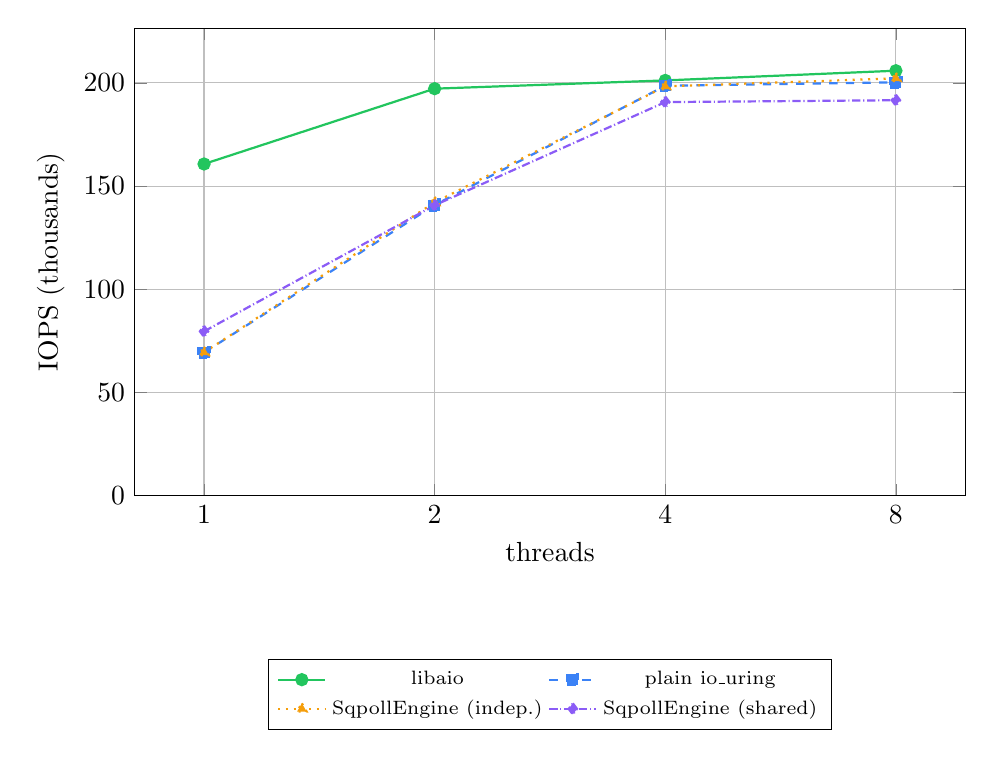
\begin{tikzpicture}
\begin{axis}[
    width=\linewidth,
    height=0.62\linewidth,
    xmode=log,
    log basis x=2,
    xtick={1,2,4,8},
    xticklabels={1,2,4,8},
    xlabel={threads},
    ylabel={IOPS (thousands)},
    ymin=0,
    grid=major,
    legend style={font=\scriptsize, at={(0.5,-0.35)}, anchor=north, legend columns=2},
]
\addplot[color=cLibaio, mark=*, thick] coordinates {(1,160.7)(2,197.2)(4,201.2)(8,205.9)};
\addlegendentry{libaio}
\addplot[color=cPlainUring, mark=square*, dashed, thick]
    coordinates {(1,69.3)(2,140.8)(4,198.6)(8,200.3)};
\addlegendentry{plain io\_uring}
\addplot[color=cSqpollIndep, mark=triangle*, dotted, thick]
    coordinates {(1,69.4)(2,142.1)(4,198.3)(8,202.2)};
\addlegendentry{SqpollEngine (indep.)}
\addplot[color=cSqpollShared, mark=diamond*, densely dashdotted, thick]
    coordinates {(1,79.6)(2,140.7)(4,190.7)(8,191.6)};
\addlegendentry{SqpollEngine (shared)}
\end{axis}
\end{tikzpicture}
\caption{IOPS versus thread count at queue depth 32, 16 vCPUs (Table~\ref{tab:16vcpu-qd32}).
\texttt{libaio}'s lead is widest at a single thread; every backend converges near the device
ceiling by 4 threads.}
\label{fig:iops-16vcpu}
\end{figure}

\begin{table}[t]
\centering
\caption{4 threads, queue depth 128: p99 latency (ms), 4 vCPUs vs.\ 16 vCPUs.}
\label{tab:tail-compare}
\begin{tabular}{lrr}
\toprule
Backend & 4 vCPU box & 16 vCPU box \\
\midrule
\texttt{libaio} & 14.3 & 15.1 \\
Plain \texttt{io\_uring} & 15.0 & 40.4 \\
SqpollEngine (shared poller) & 23.5 & 47.6 \\
\bottomrule
\end{tabular}
\end{table}

Tail latency moves the wrong way for the wider box to be a simple fix. Table~\ref{tab:tail-compare}
compares the same 4-thread, queue-depth-128 configuration across both machine sizes:
\texttt{SqpollEngine}'s shared-poller p99 latency is worse on 16 vCPUs (47.6\,ms) than on 4
(23.5\,ms), and plain \texttt{io\_uring}'s p99 grew substantially as well (15.0\,ms to
40.4\,ms), while \texttt{libaio}'s stayed close to unchanged (14.3\,ms to 15.1\,ms). More
available cores did not reduce the time a completion waits before it is harvested; if anything,
it increased it for both \texttt{io\_uring}-based paths.

\begin{figure}[t]
\centering
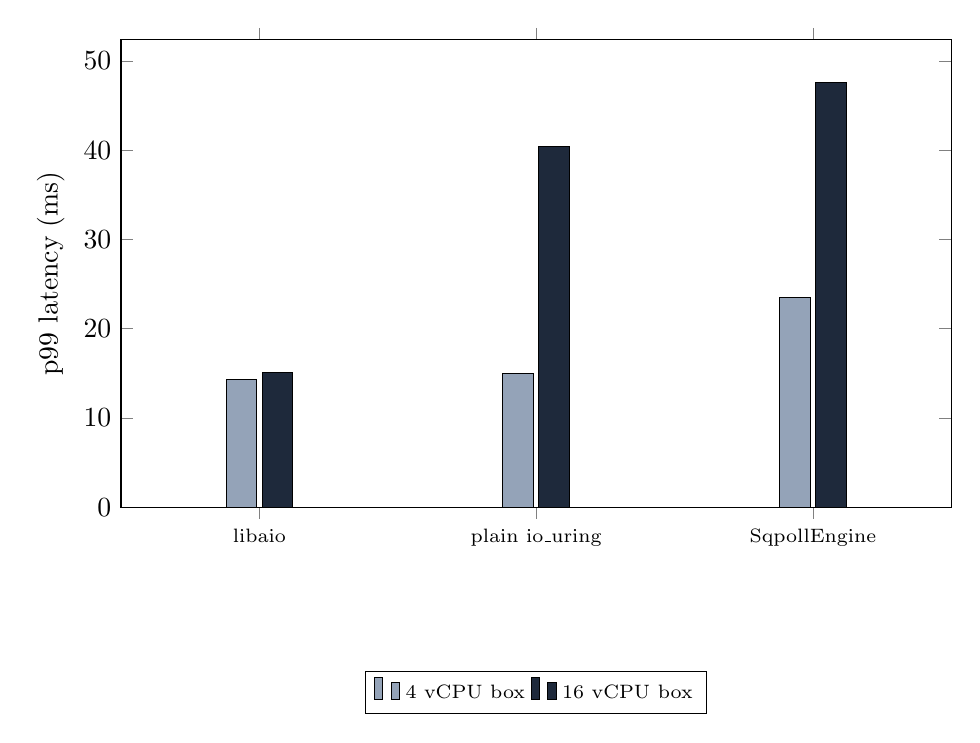
\begin{tikzpicture}
\begin{axis}[
    ybar,
    width=\linewidth,
    height=0.62\linewidth,
    symbolic x coords={libaio,plain io\_uring,SqpollEngine},
    xtick=data,
    x tick label style={font=\scriptsize},
    ylabel={p99 latency (ms)},
    ymin=0,
    bar width=11pt,
    enlarge x limits=0.25,
    legend style={font=\scriptsize, at={(0.5,-0.35)}, anchor=north, legend columns=2},
]
\addplot[fill=cBox4] coordinates {(libaio,14.3)(plain io\_uring,15.0)(SqpollEngine,23.5)};
\addlegendentry{4 vCPU box}
\addplot[fill=cBox16] coordinates {(libaio,15.1)(plain io\_uring,40.4)(SqpollEngine,47.6)};
\addlegendentry{16 vCPU box}
\end{axis}
\end{tikzpicture}
\caption{p99 latency at 4 threads, queue depth 128, 4-vCPU versus 16-vCPU box
(Table~\ref{tab:tail-compare}). \texttt{libaio}'s tail barely moves; both \texttt{io\_uring}-based
backends get worse on the wider machine.}
\label{fig:tail-compare}
\end{figure}

\section{Discussion}

The open question from Section~V-B is answered in the negative: SQPOLL's IOPS shortfall against
\texttt{libaio} and plain \texttt{io\_uring} is not a core-budget artifact of the smaller test
machine, since widening the core count did not close it and in \texttt{libaio}'s case widened it.
What remains open is why.

One candidate explanation is that \texttt{SqpollEngine}'s completion-harvesting path, a
non-blocking peek of the CQ followed by application-side backoff when it finds nothing, scales
worse than \texttt{libaio}'s blocking \texttt{io\_getevents} or plain \texttt{io\_uring}'s
\texttt{io\_uring\_wait\_cqe\_nr} at higher core counts, because a busy-waiting or
backoff-looping application thread and a busy-spinning kernel poller thread contend for shared
cache lines on the completion ring more as more cores are involved. This is a plausible
mechanism, consistent with the tail-latency data in Table~\ref{tab:tail-compare}, but this suite
did not instrument cache-coherence traffic, memory-controller counters, or per-core cycle
accounting, so we report it as a hypothesis this data is consistent with, not as a confirmed
cause. A second, unexplored candidate is that the fixed \texttt{sq\_thread\_idle} and
completion-side backoff parameters used throughout this study were tuned, informally, against
the 4-vCPU box and never retuned for 16; poller-idle and backoff tuning specific to the wider
box is the only avenue in this investigation's plan that remains untried.

We do not treat either candidate as established. The honest summary of what this suite's data
supports is: SQPOLL trades throughput and tail latency for a large reduction in kernel entries
per operation, and that trade does not improve, and by one measure gets worse, on a machine with
more spare cores.

\section{Limitations and Threats to Validity}

All measurements were taken on GCE Local SSD NVMe devices behind a virtualization layer;
absolute IOPS and latency figures reflect that layer as well as the underlying flash, and should
not be read as characterizing bare-metal NVMe performance. Every VM used \texttt{n2-standard}
machine types at a single vendor and a single fixed clock; we did not test other cloud providers,
other NVMe generations, or bare-metal hardware. The thread-count sweep for the four pipelined
backends was bounded to $\{1, 2, 4, 8\}$ rather than the full range POSIX uses, an explicit
cost-versus-coverage trade-off; a gap between 8 and higher thread counts, where the 4-vCPU box's
independent-ring collapse first became severe, is not directly re-tested at 16 vCPUs beyond 8
threads. \texttt{calls\_per\_op} is an exact syscall count for POSIX and \texttt{libaio} but only
an upper bound for the three \texttt{io\_uring}-based backends, as discussed in Section~IV-C; the
true syscall counts for those backends may be lower than reported. Each backend was measured at
its own best-practice buffer handling (\texttt{SqpollEngine}'s fixed, pre-registered buffers
against the baselines' aligned heap memory), which is the intended comparison but is not an
identical-conditions comparison in the buffer-handling dimension. Finally, the discussion in
Section~VI is explicitly not settled by this data; the cross-core contention hypothesis has not
been tested with hardware performance counters.

\section{Related Work}

Kernel-bypass and reduced-syscall I/O designs have a long history outside the storage stack
specifically. Arrakis~\cite{arrakis} and IX~\cite{ix} moved network I/O out of the kernel's
control-plane path entirely, arguing, as we do here for storage, that per-operation kernel
crossings dominate cost once device latency drops far enough. The Storage Performance
Development Kit~\cite{spdk} takes this further for NVMe specifically, running the entire driver
in user space with no kernel involvement in the data path at all, a stronger design point than
SQPOLL, which still routes I/O through the kernel's block layer but removes the per-operation
syscall. \texttt{io\_uring} itself, and the SQPOLL mode this paper evaluates, are described in
Axboe's original design document~\cite{axboe-io-uring}; \texttt{libaio}'s interface is documented
in the Linux man-pages project~\cite{aio-manpages}. Where this paper differs from prior
descriptions of \texttt{io\_uring}'s design intent is in reporting where an implementation built
around that intent actually lands empirically against its intended baselines, including a
negative result on raw throughput and the measurement pitfalls that produced misleading numbers
along the way.

\section{Conclusion}

We built \texttt{ringio} around the argument that an SQPOLL kernel poller, by removing the
per-operation syscall other asynchronous I/O interfaces still pay, should win on IOPS against
\texttt{libaio} and plain \texttt{io\_uring} on real NVMe. Measured across two machine sizes and
a swept thread-count and queue-depth matrix, it does not. \texttt{libaio} matches or beats every
SQPOLL configuration we tested on raw IOPS at every point in the matrix, and its advantage grows,
not shrinks, on a wider-core machine, ruling out core oversubscription as the explanation.
SQPOLL's actual advantage, an order-of-magnitude reduction in kernel entries per completed
operation at high queue depth, comes with a tail-latency cost that also grows on the wider
machine rather than shrinking. The underlying mechanism for that growth remains open; this paper
reports what was measured and separates it plainly from what was not.

\begin{thebibliography}{9}

\bibitem{arrakis}
S.~Peter, J.~Li, I.~Zhang, D.~R.~K.~Ports, D.~Woos, A.~Krishnamurthy, T.~Anderson, and
T.~Roscoe, ``Arrakis: The operating system is the control plane,'' \textit{ACM Transactions on
Computer Systems}, vol.~33, no.~4, 2015.

\bibitem{ix}
A.~Belay, G.~Prekas, A.~Klimovic, S.~Grossman, C.~Kozyrakis, and E.~Bugnion, ``IX: A protected
dataplane operating system for high throughput and low latency,'' in \textit{Proceedings of the
11th USENIX Symposium on Operating Systems Design and Implementation (OSDI)}, 2014.

\bibitem{spdk}
Storage Performance Development Kit (SPDK), Intel Corporation and SPDK contributors,
\url{https://spdk.io}.

\bibitem{axboe-io-uring}
J.~Axboe, ``Efficient IO with io\_uring,'' Linux kernel documentation,
\url{https://kernel.dk/io_uring.pdf}.

\bibitem{aio-manpages}
Linux man-pages project, \texttt{io\_submit(2)}, \texttt{io\_getevents(2)}, and
\texttt{io\_uring\_enter(2)} manual pages, \url{https://man7.org}.

\end{thebibliography}

\end{document}
